\subsection{Analysis}
\label{sec:analysis}

We focus our analysis on two aspects of mobile-agent interaction: how environment coverage relates to transfer, and how app-native tools contribute to task completion.



\begin{figure*}[h]
\centering
\begin{minipage}[t]{0.39\textwidth}
\centering
\vspace{0pt}
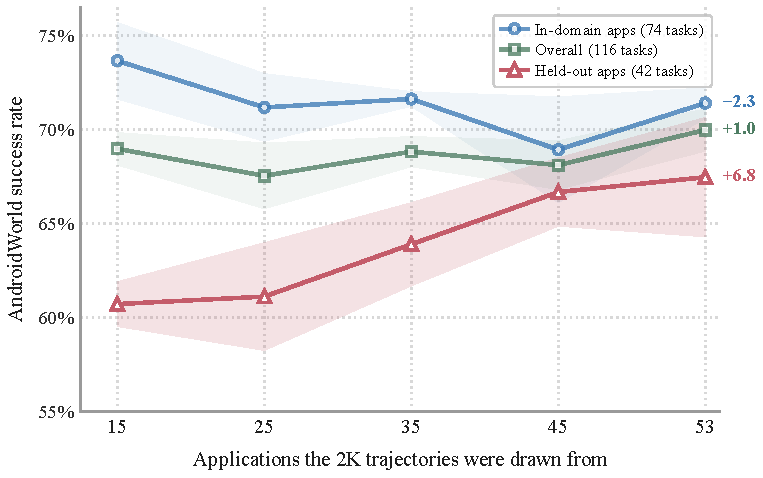
\includegraphics[width=\linewidth]{figures/exp-env-scaling.pdf}\\[-0.2em]
{\small (a) Environment coverage}
\end{minipage}
\hfill
\begin{minipage}[t]{0.59\textwidth}
\centering
\vspace{0pt}
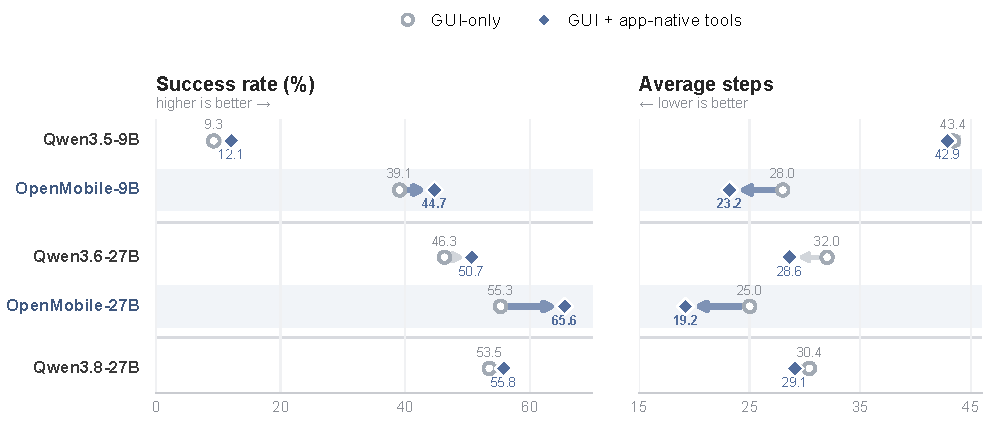
\includegraphics[width=\linewidth]{figures/exp-tool-analysis.pdf}\\[-0.2em]
{\small (b) App-native tool use}
\end{minipage}
\caption{
\textbf{Environment coverage and app-native tool use.}
(a)~Broader coverage improves held-out AndroidWorld performance at a fixed 2K-trajectory budget.
(b)~App-native tools improve success and efficiency, with larger gains after Hybrid SFT.
}
\label{fig:analysis-results}
\end{figure*}


\paragraph{Broader environment coverage improves transfer under a fixed data budget.}
A key question is whether mobile-agent experience benefits more from depth within a few applications or breadth across many applications. We fix the backbone, optimizer, and total training data at 2K emulator trajectories, and vary only the number of applications covered, from 15 to 53; all settings include the same 15 in-distribution (InD) applications. Two observations follow. First, broader coverage improves transfer: Pass@1 on unseen applications rises from 60.7 to 67.5 as coverage grows (Figure~\ref{fig:analysis-results}a). Since the data budget is fixed, this gain comes from breadth rather than from more trajectories. Second, InD performance is maintained even as InD data shrinks. Because the budget is shared, every added application takes trajectories away from the InD applications, and their data share falls from 100\% to 39.1\% (Table~\ref{tab:env-split}); yet InD Pass@1 changes only from 73.7 to 71.4. These results suggest that application coverage provides an additional scaling dimension for mobile-agent experience, with broader coverage improving transfer without substantially compromising performance on familiar applications.


\begin{table}[h]
\centering
\small
\begin{minipage}[t]{0.33\linewidth}
\centering
\caption{Environment-coverage settings under a fixed budget of 2K trajectories. InD data share is the fraction of training trajectories collected in the 15 in-distribution applications shared by all settings.}
\label{tab:env-split}
\setlength{\tabcolsep}{3pt}
\begin{tabular}{cc}
\toprule
\# Train apps & InD data share \\
\midrule
15 & 100\% \\
25 & 64.0\% \\
35 & 48.9\% \\
45 & 41.1\% \\
53 & 39.1\% \\
\bottomrule
\end{tabular}
\end{minipage}
\hfill
\begin{minipage}[t]{0.63\linewidth}
\centering
\caption{\textbf{App-native tool use on MobileGym++.}
TR (tool-call rate) is the average number of app-native tool calls per task, while TSR (tool success rate) is the fraction of tool calls that execute successfully. \#Tools is the number of distinct tools invoked across the benchmark, and \#Tasks is the number of tasks (out of 215) in which at least one app-native tool is called.}


\label{tab:tool_use}
\setlength{\tabcolsep}{3pt}
\begin{tabular}{llcccc}
\toprule
Model & Stage & TR & TSR & \#Tools & \#Tasks \\
\midrule
% Qwen3.8-27B & Base & 0.49 & 99\% & \tbd{} & \tbd{} \\
GUI-Owl-1.5-8B &- &0.58&49\%&15&20\\
GUI-Owl-1.5-32B &- &0.51&78\%&51&45\\
\midrule
\multirow{2}{*}{Qwen3.5-9B} & Base & 0.64 & 94\% & 28 & 21 \\
 & + Hybrid SFT & 1.41 & 78\% & 110 & 113 \\
\midrule
\multirow{2}{*}{Qwen3.6-27B} & Base & 1.64 & 86\% & 97 & 102 \\
 & + Hybrid SFT & 2.23 & 81\% & 115 & 128 \\
\bottomrule
\end{tabular}
\end{minipage}
\end{table}




\paragraph{Hybrid GUI--tool interaction shows substantial untapped potential.}

Simply exposing app-native tools already helps models complete mobile tasks, but existing GUI-only models use them conservatively and capture only a fraction of their potential benefit. Without hybrid training, tool calls occur in only 20--102 of the 215 tasks (Table~\ref{tab:tool_use}), and the resulting improvement remains modest: even the strongest GUI-only baseline gains only 2.3 points from tool access, while no model saves more than 3.4 steps (Figure~\ref{fig:analysis-results}b). Hybrid SFT substantially changes how models exploit the expanded action space. Tool calls increase to 113 and 128 tasks and cover 110 and 115 distinct tools. Although this increased tool usage does not immediately translate into uniformly higher success rates, as models can still make tool-use errors such as selecting unfamiliar tools or providing incorrect arguments, the trained models become substantially more effective when they do use tools. The tool-enabled gain rises to 5.6 points for the 9B model and 10.3 points for the 27B model, while trajectories become 4.8 and 5.8 steps shorter, respectively. This gap between tool availability and effective tool utilization suggests that the main bottleneck is not access to the expanded action space, but learning when, which, and how to invoke tools alongside GUI actions. More broadly, these results suggest that hybrid GUI--tool interaction offers substantial untapped potential: improving models' ability to decide when, which, and how to invoke native tools could unlock further gains from the combined action space.